% ============================================================
%  يُترجَم بـ XeLaTeX  (في Overleaf: Menu → Compiler → XeLaTeX)
%  الخط: Amiri (متوفر في Overleaf، أو حمّله من github.com/aliftype/amiri)
% ============================================================
\documentclass[12pt,a4paper]{article}
\usepackage[a4paper,margin=1.7cm,top=2.3cm,bottom=2.9cm,headheight=15pt,footskip=1.5cm]{geometry}
\usepackage{amsmath,amssymb}
\usepackage{icomma}
\usepackage[english,bidi=default,layout=lists]{babel}
\babelprovide[import,main]{arabic}
\babelfont{rm}[Scale=1.08]{Amiri}
\babelfont{sf}[Scale=1.08]{Amiri}
\usepackage[most]{tcolorbox}
\usepackage{tikz}
\usetikzlibrary{arrows.meta,calc,shadings}
\usepackage{array}
\usepackage{colortbl}
\usepackage{fancyhdr}
\usepackage{titlesec}
\usepackage{enumitem}
\usepackage{collcell}
\usepackage{needspace}
\usepackage{etoolbox}
\newcolumntype{C}{>{\collectcell\ar}c<{\endcollectcell}}
\pretocmd{\section}{\Needspace{15\baselineskip}}{}{}
\pretocmd{\subsection}{\Needspace{11\baselineskip}}{}{}

\definecolor{cDef}{HTML}{1F4E9C}
\definecolor{cThm}{HTML}{B3261E}
\definecolor{cRem}{HTML}{2E7D32}
\definecolor{cEx}{HTML}{C76B00}
\definecolor{cMeth}{HTML}{6A1B9A}
\definecolor{cSol}{HTML}{00695C}
\definecolor{cSec}{HTML}{1F3A68}

\titleformat{\section}{\Large\bfseries\color{cSec}}{\thesection.}{0.6em}{}[{\color{cSec!60}\titlerule[1pt]}]
\titleformat{\subsection}{\large\bfseries\color{cThm!85!black}}{\thesubsection.}{0.5em}{}
\titlespacing*{\section}{0pt}{14pt}{8pt}
\titlespacing*{\subsection}{0pt}{10pt}{5pt}
\setlength{\parindent}{0pt}
\setlength{\parskip}{4pt}
\setlist{itemsep=2pt,topsep=3pt}

\newtcolorbox{arbox}[3][]{enhanced,
  colback=#2!5,colframe=#2!80!black,arc=2mm,boxrule=0.8pt,
  left=6pt,right=6pt,top=8pt,bottom=5pt,
  fonttitle=\bfseries,coltitle=white,
  title={\foreignlanguage{arabic}{#3}},
  attach boxed title to top right={xshift=-5mm,yshift=-3mm},
  boxed title style={colback=#2!80!black,arc=1.5mm,boxrule=0pt},
  before upper={\selectlanguage{arabic}},
  before skip=8pt,after skip=8pt,breakable,#1}
\newenvironment{BOX}[2]{\begin{otherlanguage}{english}\begin{arbox}{#1}{#2}}{\end{arbox}\end{otherlanguage}}
\newenvironment{tarif}[1][تعريف]{\begin{BOX}{cDef}{#1}}{\end{BOX}}
\newenvironment{khassia}[1][خاصية]{\begin{BOX}{cThm}{#1}}{\end{BOX}}
\newenvironment{molahada}[1][ملاحظة]{\begin{BOX}{cRem}{#1}}{\end{BOX}}
\newenvironment{mithal}[1][مثال]{\begin{BOX}{cEx}{#1}}{\end{BOX}}
\newenvironment{tariqa}[1][طريقة]{\begin{BOX}{cMeth}{#1}}{\end{BOX}}

\newcounter{exo}
\newenvironment{tamrin}[1]{\stepcounter{exo}\begin{BOX}{cSec}{التمرين \theexo: #1}}{\end{BOX}}
\newenvironment{hal}{\Needspace{12\baselineskip}\begin{otherlanguage}{english}\begin{arbox}[breakable]{cSol}{حل التمرين \theexo}}{\end{arbox}\end{otherlanguage}}

\newenvironment{LTR}{\begin{otherlanguage}{english}}{\end{otherlanguage}}
\newcommand{\ar}[1]{\foreignlanguage{arabic}{#1}}

\renewcommand{\dots}{\mathinner{\ldotp\ldotp\ldotp}}
\renewcommand{\ldots}{\mathinner{\ldotp\ldotp\ldotp}}
\renewcommand{\cdots}{\mathinner{\cdotp\cdotp\cdotp}}
\newcommand{\N}{\mathbb{N}}
\newcommand{\Z}{\mathbb{Z}}
\newcommand{\D}{\mathbb{D}}
\newcommand{\Q}{\mathbb{Q}}
\newcommand{\R}{\mathbb{R}}
\newcommand{\pgcd}{\operatorname{PGCD}}
\newcommand{\ppcm}{\operatorname{PPCM}}

% \NLseg{a}{b}{[}{]} ; \NLright{a}{[} ; \NLleft{b}{]}  (interval on a number line)
\newcommand{\NLseg}[4]{\begin{LTR}\begin{tikzpicture}[baseline=-0.6ex]
 \draw[-{Stealth[length=2mm]},gray!70](0,0)--(3.4,0);
 \draw[line width=2pt,cThm!80!black](0.7,0)--(2.7,0);
 \node[cThm!80!black,font=\LARGE] at (0.7,0){$#3$};
 \node[cThm!80!black,font=\LARGE] at (2.7,0){$#4$};
 \node[below=3pt,font=\footnotesize] at (0.7,0){$#1$};
 \node[below=3pt,font=\footnotesize] at (2.7,0){$#2$};
\end{tikzpicture}\end{LTR}}
\newcommand{\NLright}[2]{\begin{LTR}\begin{tikzpicture}[baseline=-0.6ex]
 \draw[-{Stealth[length=2mm]},gray!70](0,0)--(3.4,0);
 \draw[line width=2pt,cThm!80!black](1.3,0)--(3.3,0);
 \node[cThm!80!black,font=\LARGE] at (1.3,0){$#2$};
 \node[below=3pt,font=\footnotesize] at (1.3,0){$#1$};
\end{tikzpicture}\end{LTR}}
\newcommand{\NLleft}[2]{\begin{LTR}\begin{tikzpicture}[baseline=-0.6ex]
 \draw[-{Stealth[length=2mm]},gray!70](0,0)--(3.4,0);
 \draw[line width=2pt,cThm!80!black](0.05,0)--(2.1,0);
 \node[cThm!80!black,font=\LARGE] at (2.1,0){$#2$};
 \node[below=3pt,font=\footnotesize] at (2.1,0){$#1$};
\end{tikzpicture}\end{LTR}}

% ---------- social-media icons (pure TikZ) ----------
\definecolor{cFB}{HTML}{1877F2}
\definecolor{cTG}{HTML}{229ED9}
\definecolor{cIG1}{HTML}{FEDA75}
\definecolor{cIG2}{HTML}{D62976}
\definecolor{cIG3}{HTML}{4F5BD5}
\newcommand{\fbicon}{\begin{LTR}\begin{tikzpicture}[baseline=-0.75ex,x=1em,y=1em]
 \fill[cFB] (0,0) circle (0.55);
 \node[white,inner sep=0,font=\usefont{TU}{lmss}{bx}{n}\small] at (0.04,-0.02) {f};
\end{tikzpicture}\end{LTR}}
\newcommand{\igicon}{\begin{LTR}
\begin{tikzpicture}[baseline=-0.75ex,x=1em,y=1em]
 \shade[lower left=cIG1,lower right=cIG2,upper left=cIG2,upper right=cIG3,rounded corners=0.28em] (-0.55,-0.55) rectangle (0.55,0.55);
 \draw[white,line width=0.09em,rounded corners=0.18em] (-0.36,-0.36) rectangle (0.36,0.36);
 \draw[white,line width=0.09em] (0,0) circle (0.17);
 \fill[white] (0.22,0.22) circle (0.05);
\end{tikzpicture}\end{LTR}}
\newcommand{\tgicon}{\begin{LTR}
\begin{tikzpicture}[baseline=-0.75ex,x=1em,y=1em]
 \fill[cTG] (0,0) circle (0.55);
 \fill[white] (-0.33,0.0) -- (0.32,0.27) -- (0.2,-0.3) -- (0.0,-0.15) -- (-0.08,-0.28) -- (-0.08,-0.08) -- cycle;
 \fill[cTG!70!black] (-0.08,-0.08) -- (0.25,0.2) -- (0.0,-0.15) -- (-0.08,-0.28) -- cycle;
\end{tikzpicture}\end{LTR}}
% page number: black box, white two-digit number, at the right of the social row
\newcommand{\PageBox}{\begin{LTR}\tikz[baseline=(p.base)]\node[fill=black,text=white,inner sep=2.5pt,minimum width=1.6em,minimum height=1.3em,font=\usefont{TU}{lmss}{bx}{n}\small](p){\ifnum\value{page}<10 0\fi\arabic{page}};\end{LTR}}
% visual left-to-right order: Telegram | Instagram | Facebook | page box
\newcommand{\SocialRow}{\begin{otherlanguage}{english}%
 \ar{\textbf{الأستاذ سوايسية هشام للرياضيات}}\ \tgicon\hfill
 \textbf{prof\_hicham\_math}\ \igicon\hfill
 \ar{\textbf{الأستاذ سوايسية هشام للرياضيات}}\ \fbicon\hspace{2.2em}\PageBox\end{otherlanguage}}

\pagestyle{fancy}
\fancyhf{}
\renewcommand{\headrulewidth}{0.6pt}
\renewcommand{\footrulewidth}{0.4pt}
% \SetHeader{right head: document title}{left head: level -- stream}
\newcommand{\SetHeader}[2]{%
 \fancyhead[C]{\parbox{\textwidth}{\ar{#1\hfill #2}}}%
 \fancyfoot[C]{\parbox{\textwidth}{\small\SocialRow}}}
\usepackage{tkz-tab}
\usepackage{multicol}
% variation / sign table (LTR)
\newenvironment{TAB}{\par\begin{center}\begin{LTR}\begin{tikzpicture}[scale=0.95,every node/.style={font=\small}]}{\end{tikzpicture}\end{LTR}\end{center}}
% grid + axes, clipped: \begin{GR}{xmin}{xmax}{ymin}{ymax}{unit cm}
\newenvironment{GR}[5]{\par\begin{center}\begin{LTR}\begin{tikzpicture}[x=#5cm,y=#5cm,font=\footnotesize]
 \draw[gray!25,very thin] (#1,#3) grid (#2,#4);
 \draw[-{Stealth[length=2mm]}] (#1,0)--(#2+0.3,0) node[below left]{$x$};
 \draw[-{Stealth[length=2mm]}] (0,#3)--(0,#4+0.3) node[below left]{$y$};
 \node[below left] at (0,0){$O$};
 \begin{scope}\clip (#1,#3) rectangle (#2,#4);}
{\end{scope}\end{tikzpicture}\end{LTR}\end{center}}
\newcommand{\Ticks}[2]{\foreach \t in {#1} \node[below,font=\scriptsize] at (\t,0){$\t$}; \foreach \t in {#2} \node[left,font=\scriptsize] at (0,\t){$\t$};}
\newcommand{\bx}[1]{\ensuremath{\colorbox{cDef!12}{$\displaystyle #1$}}}
\newcommand{\TwoCol}[4]{\par\begin{LTR}\noindent\begin{minipage}[t]{#1\textwidth}\selectlanguage{arabic}#2\end{minipage}\hfill\begin{minipage}[t]{#3\textwidth}\selectlanguage{arabic}#4\end{minipage}\end{LTR}\par}
\newcommand{\RL}[4]{\TwoCol{#3}{#4}{#1}{#2}}  % \RL{w1}{right content}{w2}{left content}
\newcommand{\ok}{$\textcolor{cRem}{\checkmark}$}
\newcommand{\limn}{\displaystyle\lim_{n\to+\infty}}
% sub-questions, each on its own line
\newenvironment{sq}{\begin{itemize}[leftmargin=2.4em,itemsep=3pt]}{\end{itemize}}
\newcommand{\qa}{\item[(أ)]}\newcommand{\qb}{\item[(ب)]}\newcommand{\qc}{\item[(جـ)]}\newcommand{\qd}{\item[(د)]}\newcommand{\qe}{\item[(هـ)]}
\newcommand{\pa}{\par\smallskip\textbf{(أ)} }\newcommand{\pb}{\par\smallskip\textbf{(ب)} }\newcommand{\pc}{\par\smallskip\textbf{(جـ)} }\newcommand{\pd}{\par\smallskip\textbf{(د)} }\newcommand{\pe}{\par\smallskip\textbf{(هـ)} }
\newcommand{\QQ}[1]{\par\smallskip\textbf{#1.} }
\newenvironment{tmr}{\stepcounter{exo}\begin{BOX}{cSec}{تمرين محلول \theexo}}{\end{BOX}}
\newcommand{\ABC}[3]{\\[2pt]\begin{tabular}{p{0.28\textwidth}p{0.28\textwidth}p{0.28\textwidth}}(جـ) \ #3 & (ب) \ #2 & (أ) \ #1\end{tabular}}
\pretocmd{\section}{\Needspace{24\baselineskip}}{}{}
\newtcbox{\bxtbox}{on line,colback=cDef!12,colframe=cDef!12,boxrule=0pt,arc=1pt,boxsep=0pt,left=2pt,right=2pt,top=1pt,bottom=1pt}
\newcommand{\bxt}[1]{\foreignlanguage{english}{\bxtbox{\ar{#1}}}}
\usepackage{longtable}
\setlength{\LTpre}{4pt}\setlength{\LTpost}{0pt}
\newcommand{\Phase}[1]{\textbf{#1}}
\newcommand{\Fld}[2]{\textbf{#1:}\ #2}
% رأس المذكرة على نمط النموذج: إطار بعنوان «مذكرة رقم»، معلومات الحصة، ثم إطار الكفاءات
\newcommand{\ModhHead}[9]{%
\begin{LTR}
\begin{tcolorbox}[enhanced,colback=white,colframe=cThm!85!black,arc=4mm,boxrule=1pt,top=14pt,bottom=6pt,left=8pt,right=8pt,
 overlay={\node[fill=cThm!85!black,text=white,rounded corners=3mm,inner xsep=14pt,inner ysep=4pt,font=\large\bfseries] at ([yshift=0pt]frame.north){\ar{مذكرة رقم #1}};},
 before upper={\selectlanguage{arabic}}]
\begin{tabular}{@{}p{0.4\linewidth}p{0.55\linewidth}@{}}
\Fld{المستوى}{#2} & \Fld{الثانوية}{\dotfill}\\[3pt]
\Fld{المادة}{رياضيات} & \Fld{ميدان التعلم}{#3}\\[3pt]
\Fld{المدة}{#5} & \Fld{الوحدة التعلمية}{#4}\\[3pt]
\Fld{الأستاذ}{\dotfill} & \Fld{المحتوى المعرفي}{#6}\\
\end{tabular}
\end{tcolorbox}
\begin{tcolorbox}[enhanced,colback=white,colframe=cThm!85!black,arc=3mm,boxrule=0.8pt,sidebyside,sidebyside align=top,lefthand ratio=0.5,
 segmentation style={dashed,cThm!60},before upper={\selectlanguage{arabic}},before lower={\selectlanguage{arabic}}]
\textbf{الكفاءات المستهدفة:}\par #8
\tcblower
\textbf{الكفاءات القبلية:}\par #7
\end{tcolorbox}
\end{LTR}
\par\smallskip\textbf{الوسائل:} #9\par\smallskip}
\newenvironment{Sayr}{%
\begin{LTR}\renewcommand{\arraystretch}{1.25}
\begin{longtable}{|p{0.17\textwidth}|>{\centering\arraybackslash}p{0.06\textwidth}|p{0.53\textwidth}|>{\centering\arraybackslash}p{0.12\textwidth}|}
\hline\rowcolor{cThm!12}\ar{\textbf{توجيهات وتعاليق}} & \ar{\textbf{المدة}} & \ar{\textbf{سير الحصة}} & \ar{\textbf{مراحل الحصة}}\\\hline\endhead
\hline\endfoot}{\end{longtable}\end{LTR}}
% سطر في الجدول: \Row{مرحلة}{سير}{مدة}{توجيهات}
\newcommand{\Row}[4]{\ar{\small #4} & \ar{#3} & \ar{#2} & \cellcolor{cThm!8}\ar{\Phase{#1}}\\\hline}

\newcommand{\Lab}[2]{\foreignlanguage{english}{\tcbox[on line,colback=#1,colframe=#1,boxrule=0pt,arc=2pt,boxsep=1pt,left=5pt,right=5pt,top=1pt,bottom=1pt]{\ar{\textcolor{white}{\textbf{#2}}}}}}
\newcommand{\Num}[1]{\foreignlanguage{english}{\tikz[baseline=(c.base)]\node[fill=cDef,text=white,inner sep=2pt,font=\footnotesize\bfseries](c){#1};}}
\newcommand{\ck}{\ensuremath{{\color{cRem}\checkmark}}}
\newenvironment{Kad}[1]{\par\smallskip\Lab{#1}}{\par}
\SetHeader{\small\bfseries\color{cSec}مذكرات محور: الاشتقاقية والاستمرارية}{\small\color{cSec}السنة الثالثة ثانوي -- تسيير واقتصاد}
\begin{document}
\begin{LTR}
\begin{tcolorbox}[enhanced,colback=cThm!85!black,colframe=cThm!85!black,arc=3mm,halign=center,boxrule=0pt,top=12pt,bottom=12pt,before upper={\selectlanguage{arabic}}]
{\color{white}\fontsize{24}{30}\selectfont\bfseries مذكرات محور: الاشتقاقية والاستمرارية}\\[8pt]
{\color{white}\large السنة الثالثة ثانوي -- تسيير واقتصاد}\\[4pt]
{\color{white}\large 6 مذكرات (12 ساعة) -- السنة الدراسية 2026-2027}
\end{tcolorbox}
\end{LTR}
\begin{BOX}{cThm}{يتضمن هذا العمل}
\begin{enumerate}[label=\textbf{مذكرة \arabic{enumi}:},leftmargin=6em,start=9]
\item العدد المشتق ، المماس (تذكير وقراءة بيانية).
\item الدوال المشتقة للدوال المرجعية ، العمليات على المشتقات.
\item المشتقات واتجاه التغير ، القيم الحدية المحلية.
\item تطبيقات اقتصادية: التكلفة المتوسطة والحدية ، الربح.
\item مركب دالتين: التعرف ، النهاية ، الاشتقاق.
\item الاستمرارية ، مبرهنة القيم المتوسطة.
\end{enumerate}
مراجع: الكتاب المدرسي للسنة الثالثة ثانوي تسيير واقتصاد (باب الاشتقاقية والاستمرارية). دراسة الدوال الكاملة في محور النهايات الموالي.
\end{BOX}
\newpage
\ModhHead{09}{3 ت ا}{تحليل}{الاشتقاقية والاستمرارية}{02 سا}{العدد المشتق ، المماس (تذكير وقراءة بيانية)}%
{\begin{itemize}\item الاشتقاقية (2 ت ا).\end{itemize}}%
{\begin{itemize}\item حساب العدد المشتق وقراءته بيانياً ، وكتابة معادلة المماس.\end{itemize}}%
{المنهاج ، الكتاب المدرسي ، مراجع ، الحاسبة البيانية.}
\begin{Sayr}
\Row{مرحلة الانطلاق}{%
\textbf{التهيئة النفسية:} ما معنى العدد المشتق هندسياً؟}{10 د}{تقويم تشخيصي.}
\Row{التشخيص والاكتشاف}{%
\Lab{cEx}{مناقشة نشاط 01 (باب الاشتقاقية)}\par\ck\ قراءة أعداد مشتقة من معاملات توجيه مماسات مرسومة.\par
\ck\ حساب عدد مشتق بنسبة التزايد.\par
}{35 د}{قراءة بيانية.}
\Row{بناء المعارف}{%
\Lab{cThm}{تذكير}\ $f^{\prime}(a)=\lim\limits_{h\to0}\dfrac{f(a+h)-f(a)}h$ ؛ المماس عند $A(a;f(a))$: $y=f^{\prime}(a)(x-a)+f(a)$.\par\Lab{cEx}{مثال}\ $f(x)=x^2-3x+1$ عند $2$: $f(2)=-1$ ، $f^{\prime}(2)=1$: المماس $y=x-3$.\par}{50 د}{المعادلة خطوة خطوة.}
\Row{}{%
\Lab{cRem}{ملاحظات}\ بيانياً: $f^{\prime}(a)$ معامل توجيه المماس عند النقطة ذات الفاصلة $a$.\par\Lab{cThm!80!black}{حذار}\ المماس الأفقي يوافق $f^{\prime}(a)=0$.}{}{}
\Row{التقويم}{%
\Lab{cEx}{تطبيق}\par اكتب معادلة مماس منحني $f(x)=\dfrac1x$ عند النقطة ذات الفاصلة $1$.\par\textbf{الحل:} $f(1)=1$ ، $f^{\prime}(1)=-1$: $y=-x+2$.\par\textbf{واجب منزلي:} تمارين من باب الاشتقاقية.\par\smallskip\textbf{ملاحظات حول سير الحصة:} \dotfill}{25 د}{تقويم فردي.}
\end{Sayr}
\newpage
\ModhHead{10}{3 ت ا}{تحليل}{الاشتقاقية والاستمرارية}{02 سا}{الدوال المشتقة للدوال المرجعية ، العمليات على المشتقات}%
{\begin{itemize}\item العدد المشتق.\end{itemize}}%
{\begin{itemize}\item حساب مشتقات الدوال المرجعية ومجموع وجداء وحاصل قسمة دوال.\end{itemize}}%
{المنهاج ، الكتاب المدرسي ، مراجع ، الحاسبة البيانية.}
\begin{Sayr}
\Row{مرحلة الانطلاق}{%
\textbf{التهيئة النفسية:} ما مشتقة $x^3$ ؟ و $x^n$ ؟}{10 د}{سؤال.}
\Row{التشخيص والاكتشاف}{%
\Lab{cEx}{وضعية مقترحة}\par\ck\ من $(x^2)^{\prime}=2x$ و $(x^3)^{\prime}=3x^2$: تخمين $(x^n)^{\prime}=nx^{n-1}$.\par
}{35 د}{تخمين.}
\Row{بناء المعارف}{%
\Lab{cThm}{خاصية}\par\ck\ $(x^n)^{\prime}=nx^{n-1}$ ($n$ صحيح) ؛ $\left(\dfrac1x\right)^{\prime}=-\dfrac1{x^2}$ ؛ $(\sqrt x)^{\prime}=\dfrac1{2\sqrt x}$.\par
\ck\ $(u+v)^{\prime}=u^{\prime}+v^{\prime}$ ؛ $(uv)^{\prime}=u^{\prime}v+uv^{\prime}$ ؛ $\left(\dfrac uv\right)^{\prime}=\dfrac{u^{\prime}v-uv^{\prime}}{v^2}$.\par
\Lab{cEx}{مثال}\ $f(x)=\dfrac{2x+1}{x-3}$: $f^{\prime}(x)=\dfrac{2(x-3)-(2x+1)}{(x-3)^2}=\dfrac{-7}{(x-3)^2}$.\par}{50 د}{جدول القواعد.}
\Row{}{%
\Lab{cThm!80!black}{حذار}\ $(uv)^{\prime}\neq u^{\prime}v^{\prime}$.}{}{}
\Row{التقويم}{%
\Lab{cEx}{تطبيق}\par احسب مشتقة $g(x)=x^3-6x^2+9x$.\par\textbf{الحل:} $g^{\prime}(x)=3x^2-12x+9$.\par\textbf{واجب منزلي:} تمارين من باب الاشتقاقية.\par\smallskip\textbf{ملاحظات حول سير الحصة:} \dotfill}{25 د}{تقويم فردي.}
\end{Sayr}
\newpage
\ModhHead{11}{3 ت ا}{تحليل}{الاشتقاقية والاستمرارية}{02 سا}{المشتقات واتجاه التغير ، القيم الحدية المحلية}%
{\begin{itemize}\item حساب المشتقات.\end{itemize}}%
{\begin{itemize}\item توظيف المشتقات لدراسة اتجاه تغير دالة وتعيين قيمها الحدية المحلية.\end{itemize}}%
{المنهاج ، الكتاب المدرسي ، مراجع ، الحاسبة البيانية.}
\begin{Sayr}
\Row{مرحلة الانطلاق}{%
\textbf{التهيئة النفسية:} منحنٍ يصعد ثم ينزل: ماذا نقول عن إشارة ميل مماساته؟}{10 د}{ملاحظة بيانية.}
\Row{التشخيص والاكتشاف}{%
\Lab{cEx}{وضعية مقترحة}\par\ck\ إشارة $f^{\prime}$ موجبة على الأجزاء المتزايدة ، سالبة على المتناقصة.\par
}{35 د}{جدول الإشارة.}
\Row{بناء المعارف}{%
\Lab{cThm}{خاصية}\par\ck\ $f^{\prime}>0$ على مجال: $f$ متزايدة تماماً ؛ $f^{\prime}<0$: متناقصة تماماً.\par
\ck\ إذا انعدمت $f^{\prime}$ عند $a$ مغيرة إشارتها فـ $f(a)$ قيمة حدية محلية.\par
\Lab{cEx}{مثال}\ $g(x)=x^3-6x^2+9x$: $g^{\prime}(x)=3(x-1)(x-3)$.\par\smallskip\begin{LTR}\centering 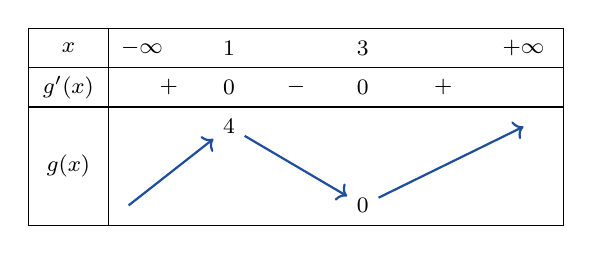
\begin{tikzpicture}[x=0.85cm,y=0.5cm,font=\footnotesize]
\draw (0,0) rectangle (8,-5); \draw (0,-1)--(8,-1); \draw (0,-2)--(8,-2); \draw (1.2,0)--(1.2,-5);
\node at (0.6,-0.5){$x$}; \node at (0.6,-1.5){$g^{\prime}(x)$}; \node at (0.6,-3.5){$g(x)$};
\node at (1.7,-0.5){$-\infty$}; \node at (3,-0.5){$1$}; \node at (5,-0.5){$3$}; \node at (7.4,-0.5){$+\infty$};
\node at (2.1,-1.5){$+$}; \node at (3,-1.5){$0$}; \node at (4,-1.5){$-$}; \node at (5,-1.5){$0$}; \node at (6.2,-1.5){$+$};
\node (a) at (3,-2.5){$4$}; \node (b) at (5,-4.5){$0$};
\draw[->,cDef,thick] (1.5,-4.5)--(a); \draw[->,cDef,thick] (a)--(b); \draw[->,cDef,thick] (b)--(7.4,-2.5);
\end{tikzpicture}\end{LTR}\par عظمى محلية $g(1)=4$ ، صغرى محلية $g(3)=0$.\par}{50 د}{جدول التغيرات.}
\Row{}{%
\Lab{cThm!80!black}{حذار}\ ندرس إشارة $f^{\prime}$ في جدول قبل الاستنتاج.}{}{}
\Row{التقويم}{%
\Lab{cEx}{تطبيق}\par $f(x)=x+\dfrac4x$ على $]0;+\infty[$: عيّن قيمتها الحدية.\par\textbf{الحل:} $f^{\prime}(x)=\dfrac{x^2-4}{x^2}$: صغرى $f(2)=4$.\par\textbf{واجب منزلي:} تمارين من باب الاشتقاقية.\par\smallskip\textbf{ملاحظات حول سير الحصة:} \dotfill}{25 د}{تقويم فردي.}
\end{Sayr}
\newpage
\ModhHead{12}{3 ت ا}{تحليل}{الاشتقاقية والاستمرارية}{02 سا}{تطبيقات اقتصادية: التكلفة المتوسطة والحدية ، الربح}%
{\begin{itemize}\item اتجاه التغير ، القيم الحدية.\end{itemize}}%
{\begin{itemize}\item توظيف المشتقات في مسائل اقتصادية (تكلفة ، إيراد ، ربح).\end{itemize}}%
{المنهاج ، الكتاب المدرسي ، مراجع ، الحاسبة البيانية.}
\begin{Sayr}
\Row{مرحلة الانطلاق}{%
\textbf{التهيئة النفسية:} مؤسسة تنتج $q$ وحدة: كيف تختار الكمية التي تجعل التكلفة المتوسطة أصغر ما يمكن؟}{10 د}{وضعية مؤسسة.}
\Row{التشخيص والاكتشاف}{%
\Lab{cEx}{وضعية مقترحة}\ التكلفة الكلية $C(q)=q^2+10q+400$ (بالألف DA) ، $q>0$.\par\ck\ التكلفة المتوسطة $C_M(q)=\dfrac{C(q)}q=q+10+\dfrac{400}q$.\par
}{35 د}{عمل بالأفواج.}
\Row{بناء المعارف}{%
\Lab{cDef}{تعريف}\ \textbf{التكلفة الحدية}: $C^{\prime}(q)$ ؛ \textbf{الإيراد}: $R(q)=p\times q$ ؛ \textbf{الربح}: $B(q)=R(q)-C(q)$.\par\Lab{cEx}{مثال}\par\ck\ $C_M^{\prime}(q)=1-\dfrac{400}{q^2}$: أصغر تكلفة متوسطة عند $q=20$ ، $C_M(20)=50$.\par
\ck\ $C^{\prime}(20)=2\times20+10=50=C_M(20)$: عند أصغر تكلفة متوسطة تتساوى التكلفتان المتوسطة والحدية.\par
\ck\ سعر البيع $70$: $B(q)=-q^2+60q-400$ ، $B^{\prime}(q)=-2q+60$: أكبر ربح $B(30)=500$.\par
}{50 د}{تفسير اقتصادي.}
\Row{}{%
\Lab{cThm!80!black}{حذار}\ نحترم مجال المتغير الاقتصادي ($q>0$).}{}{}
\Row{التقويم}{%
\Lab{cEx}{تطبيق}\par الإيراد $R(q)=q(100-2q)$ ، $0\leqslant q\leqslant50$. عيّن الكمية التي تعطي أكبر إيراد.\par\textbf{الحل:} $R^{\prime}(q)=100-4q$: $q=25$ ، $R(25)=1250$.\par\textbf{واجب منزلي:} تمارين من باب الاشتقاقية (تطبيقات اقتصادية).\par\smallskip\textbf{ملاحظات حول سير الحصة:} \dotfill}{25 د}{تقويم فردي.}
\end{Sayr}
\newpage
\ModhHead{13}{3 ت ا}{تحليل}{الاشتقاقية والاستمرارية}{02 سا}{مركب دالتين: التعرف ، النهاية ، الاشتقاق}%
{\begin{itemize}\item المشتقات ، النهايات.\end{itemize}}%
{\begin{itemize}\item التعرف على دالة كمركب دالتين بسيطتين ، وحساب نهايتها ومشتقتها.\end{itemize}}%
{المنهاج ، الكتاب المدرسي ، مراجع ، الحاسبة البيانية.}
\begin{Sayr}
\Row{مرحلة الانطلاق}{%
\textbf{التهيئة النفسية:} كيف نشتق $(3x-1)^4$ دون نشر؟}{10 د}{تحدٍّ.}
\Row{التشخيص والاكتشاف}{%
\Lab{cEx}{وضعية مقترحة}\par\ck\ $x\mapsto3x-1\mapsto(3x-1)^4$: مركب دالتين $g\circ u$.\par
}{35 د}{المخطط بالأسهم.}
\Row{بناء المعارف}{%
\Lab{cDef}{تعريف}\ $(g\circ u)(x)=g\big(u(x)\big)$.\par\Lab{cThm}{خاصية}\par\ck\ $(g\circ u)^{\prime}(x)=u^{\prime}(x)\times g^{\prime}\big(u(x)\big)$ ؛ خاصة: $(u^n)^{\prime}=nu^{\prime}u^{n-1}$ ، $(\sqrt u)^{\prime}=\dfrac{u^{\prime}}{2\sqrt u}$.\par
\ck\ إذا كان $\lim u=b$ و $\lim\limits_{X\to b}g(X)=c$ فإن $\lim g\circ u=c$.\par
}{50 د}{جدول القواعد.}
\Row{}{%
\Lab{cEx}{مثال}\ $(3x-1)^4$: مشتقتها $12(3x-1)^3$ ؛ $\sqrt{x^2+1}$: مشتقتها $\dfrac x{\sqrt{x^2+1}}$ ؛ $\lim\limits_{x\to+\infty}\sqrt{4+\frac1x}=2$.\par\Lab{cThm!80!black}{حذار}\ لا ننسى ضرب $u^{\prime}$.}{}{}
\Row{التقويم}{%
\Lab{cEx}{تطبيق}\par احسب مشتقة $h(x)=(x^2-1)^3$ ، وفكّك $k(x)=\dfrac1{2x+5}$.\par\textbf{الحل:} $6x(x^2-1)^2$ ؛ $k=g\circ u$ مع $u(x)=2x+5$ و $g(X)=\dfrac1X$.\par\textbf{واجب منزلي:} تمارين من باب الاشتقاقية.\par\smallskip\textbf{ملاحظات حول سير الحصة:} \dotfill}{25 د}{تقويم فردي.}
\end{Sayr}
\newpage
\ModhHead{14}{3 ت ا}{تحليل}{الاشتقاقية والاستمرارية}{02 سا}{الاستمرارية ، مبرهنة القيم المتوسطة}%
{\begin{itemize}\item المشتقات ، اتجاه التغير.\end{itemize}}%
{\begin{itemize}\item التعرف على دالة مستمرة ، وتطبيق مبرهنة القيم المتوسطة لإثبات وجود حل ووحدانيته.\end{itemize}}%
{المنهاج ، الكتاب المدرسي ، مراجع ، الحاسبة البيانية.}
\begin{Sayr}
\Row{مرحلة الانطلاق}{%
\textbf{التهيئة النفسية:} ربح مؤسسة سالب في البداية وموجب لاحقاً: هل توجد كمية يكون فيها الربح معدوماً؟}{10 د}{وضعية اقتصادية.}
\Row{التشخيص والاكتشاف}{%
\Lab{cEx}{وضعية مقترحة}\par\ck\ $B(q)=-q^2+60q-400$: $B(0)=-400$ ، $B(30)=500$ ، و $B$ مستمرة: يوجد $q_0$ (عتبة المردودية) حيث $B(q_0)=0$.\par
}{35 د}{قراءة بيانية.}
\Row{بناء المعارف}{%
\Lab{cThm}{خاصية}\par\ck\ كثيرات الحدود والدوال الناطقة مستمرة على كل مجال من مجموعة تعريفها.\par
\ck\ إذا كانت $f$ مستمرة على $[a;b]$ و $k$ محصوراً بين $f(a)$ و $f(b)$ فالمعادلة $f(x)=k$ تقبل حلاً على الأقل في $[a;b]$ ، وحلاً وحيداً إذا كانت $f$ رتيبة تماماً.\par
\Lab{cEx}{مثال}\ $f(x)=x^3+x-3$ على $[1;2]$: متزايدة ، $f(1)=-1$ ، $f(2)=7$: حل وحيد $\alpha$ ؛ $f(1{,}2)<0<f(1{,}3)$: $1{,}2<\alpha<1{,}3$.\par}{50 د}{جدول قيم بالحاسبة.}
\Row{}{%
\Lab{cThm!80!black}{حذار}\ المبرهنة تضمن الوجود ، والحصر بالحاسبة.}{}{}
\Row{التقويم}{%
\Lab{cEx}{تطبيق}\par بيّن أن عتبة المردودية $q_0$ في الوضعية وحيدة في $[0;30]$ ، واحصرها بسعة $1$.\par\textbf{الحل:} $B$ متزايدة على $[0;30]$ ($B^{\prime}>0$) ؛ $B(7)=-29$ ، $B(8)=16$: $7<q_0<8$.\par\textbf{واجب منزلي:} تمارين من باب الاشتقاقية والاستمرارية.\par\smallskip\textbf{ملاحظات حول سير الحصة:} \dotfill}{25 د}{نهاية المحور: فرض أو مراجعة.}
\end{Sayr}
\end{document}
